\documentclass[conference]{IEEEtran}
% \IEEEoverridecommandlockouts
% The preceding line is only needed to identify funding in the first footnote. If that is unneeded, please comment it out.
\usepackage{cite}
\usepackage{amsmath,amssymb,amsfonts}
\usepackage{algorithmic}
\usepackage{graphicx}
\usepackage{siunitx}
\usepackage{textcomp}
\usepackage{xcolor}
\def\BibTeX{{\rm B\kern-.05em{\sc i\kern-.025em b}\kern-.08em
    T\kern-.1667em\lower.7ex\hbox{E}\kern-.125emX}}
\begin{document}

\title{A Speech Recognition Model for Mandarin Chinese Pronunciation Evaluation}

\author{\IEEEauthorblockN{1\textsuperscript{st} Jakub Kiliańczyk}
\IEEEauthorblockA{\textit{Gdańsk University of Technology} \\
% \textit{name of organization (of Aff.)}\\
Gdańsk, Poland}
% \\ jacky8203@proton.me
% }
\and
\IEEEauthorblockN{2\textsuperscript{nd} Jakub Kwiatkowski}
\IEEEauthorblockA{\textit{Gdańsk University of Technology} \\
% \textit{name of organization (of Aff.)}\\
Gdańsk, Poland}
\and
\IEEEauthorblockN{3\textsuperscript{rd} Anna Strzelecka}
\IEEEauthorblockA{\textit{Gdańsk University of Technology} \\
% \textit{name of organization (of Aff.)}\\
Gdańsk, Poland}
\and
\IEEEauthorblockN{4\textsuperscript{th} Dawid Migowski}
\IEEEauthorblockA{\textit{Gdańsk University of Technology} \\
% \textit{name of organization (of Aff.)}\\
Gdańsk, Poland}
\and
\IEEEauthorblockN{5\textsuperscript{th} Łukasz Smoliński}
\IEEEauthorblockA{\textit{Gdańsk University of Technology} \\
% \textit{name of organization (of Aff.)}\\
Gdańsk, Poland}
}

\maketitle

\begin{abstract}
In recent years many Automatic Speech Recognition (ASR) solutions have been designed based on artificial intelligence algorithms. The Chinese language poses relatively new challenges when it comes to ASR or Mispronunciation Detection and Diagnosis (MDD) as the meaning of each word depends not only on pronunciation, but also on tone of speech. In order to correctly asses one's speech, both features have to be considered.
\end{abstract}

\begin{IEEEkeywords}
Automatic Speech Recognition, Mispronunciation Detection and Diagnosis, Convolutional Neural Network, Transformer
\end{IEEEkeywords}

\section{Introduction}
In order to train new Speech Recognition models, we used AISHELL-3 \cite{shi2021aishell3multispeakermandarintts} dataset and a self-made one consisting of recordings of students of Gdansk University of Technology. We developed and compared several approaches for the tasks of Speech and Scoring and Recognition and Tone Recognition.

\section{Related Work}
We conducted a literature review in search of existing research and solutions for the tasks of pronunciation and tone detection for Mandarin chinese. We specified search criteria to look for Neural Network models trained with limited data, published in years 2014-2024 in english. We based our research on the following keywords: ``Speech Recognition'', ``Deep Learning'', ``Pronunciation Evaluation'' and fetched a total of 878 research papers from several databases. After eliminating duplicates and assessing the titles and abstracts we chose 12 most suiting articles for further reading. \\
After the literature review, our first notion was the limited quantity of publicly available datasets, especially regarding the subject of Tone Classification (TC). \cite{warden2018speechcommandsdatasetlimitedvocabulary} mentions difficulties in finding and accessing datasets for ASR in Chinese and suggests a new one for Keyword Detection. We picked two Deep Learning architectures to build on and train: \cite{Gao2019ToneNetAC} (a Convolutional Neural Network - CNN), and \cite{8462506} (a Transformer).

\section{Approach}
We decided to first develop separate CNN models for the tasks of Pronunciation Evaluation (PE) and Tone Classification. Afterwards we attempted to solve both of these tasks using a Speech-Recognition architecture of a Transformer \cite{vaswani2023attentionneed,8462506}. It's possible to solve Pronunciation Scoring and Tone Classification tasks based on Speech-to-Text output in Mandarin chinese, as written chinese contains information about pronunciation and intonation. \
We trained all models with our dataset (in case of the Transformer we also used \cite{shi2021aishell3multispeakermandarintts}) and compared the results to select the most accurate approach.

\subsection{Data Processing}
In order to ensure good training quality of our dataset we applied some preprocessing techniques. Firstly, we removed the incorrect recordings, for example only constituting of noise, or ones that didn't suffice the length requirements. We decided not to use recordings shorter than 0.5s as they were mostly empty or cut in the middle of a word. We have also excluded the top 5\% of the longest recordings. We made sure not to lose data coverage of each class in the process.
We've filtered the recordings with high noise levels using the Root Mean Square (RMS) as the energy measure. We assumed a threshold of 0.004 and only left recordings with RMS above that value. We verified that the ones below were in fact too noisy to use in training. A Mel Spectrogram of such recording is presented in ``Fig.~\ref{fig_Noise}''. For comparison, ``Fig.~\ref{fig_NoNoise}'' presents a spectrogram with acceptable noise levels.

\begin{figure}[htbp]
    \centerline{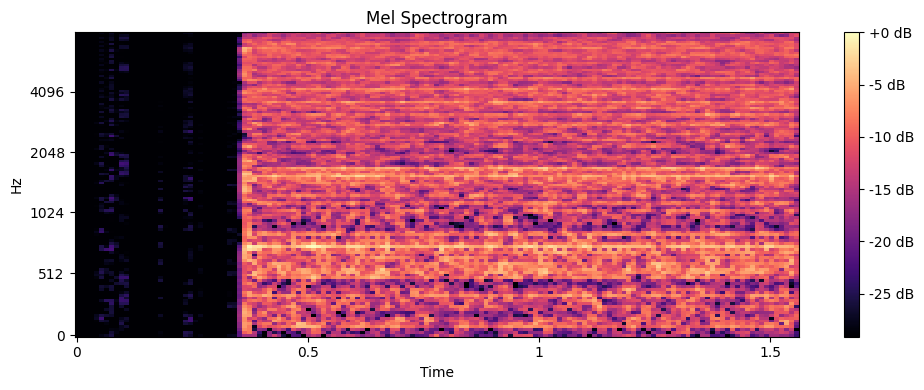
\includegraphics[width=0.5\textwidth]{Figures/Fig_Noise.png}}
    \caption{Spectrogram with high noise levels}
    \label{fig_Noise} % ``Fig.~\ref{fig_Noise}''
    \end{figure}

\begin{figure}[htbp]
    \centerline{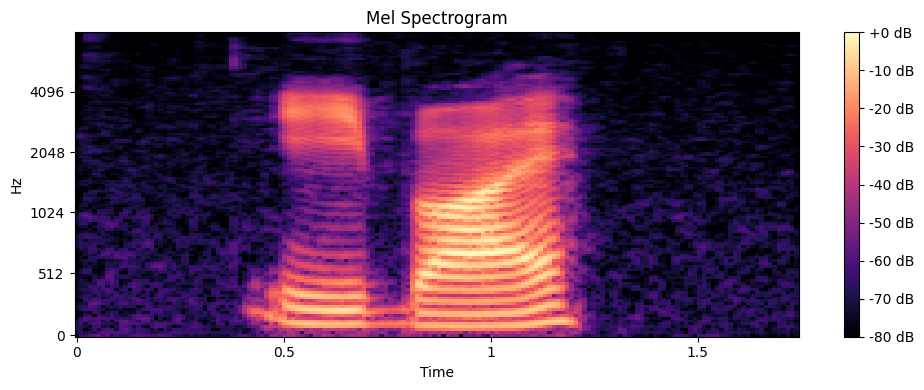
\includegraphics[width=0.5\textwidth]{Figures/Fig_NoNoise.png}}
    \caption{Spectrogram with acceptable noise levels}
    \label{fig_NoNoise} % ``Fig.~\ref{fig_Noise}''
    \end{figure}

Later, we trimmed the silent parts at the edges of the recordings and applied noise-reduction filters. The effect of trimming silent parts is shown in ``Fig.~\ref{fig_Silence}'' and ``Fig.~\ref{fig_NoSilence}''.

\begin{figure}[hbtp]
    \centerline{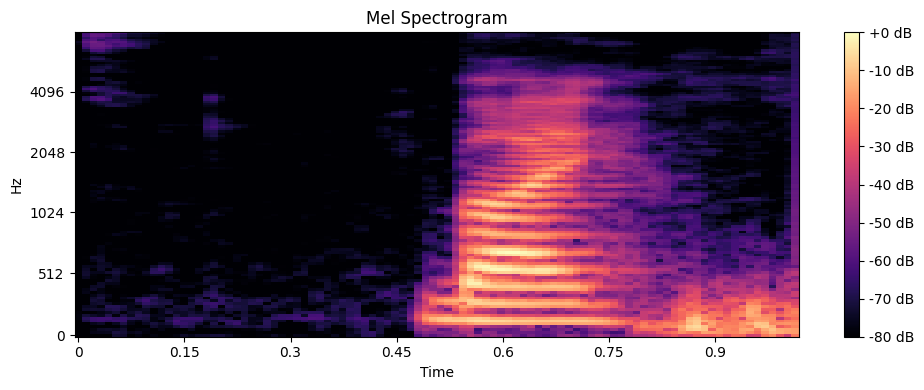
\includegraphics[width=0.5\textwidth]{Figures/Fig_Silence.png}}
    \caption{Spectrogram before trimming silent parts}
    \label{fig_Silence} % ``Fig.~\ref{fig_Noise}''
    \end{figure}

\begin{figure}[hbtp]
    \centerline{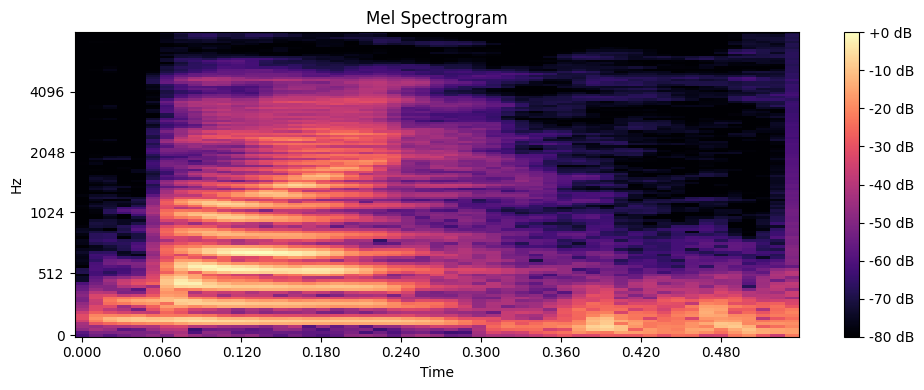
\includegraphics[width=0.5\textwidth]{Figures/Fig_NoSilence.png}}
    \caption{Spectrogram after trimming silent parts}
    \label{fig_NoSilence} % ``Fig.~\ref{fig_Noise}''
    \end{figure}

In order to reduce the noise of recordings, we applied techniques like noise profiling (based on noise from the beginning of recording), band-pass filters and spectral noise reduction.
Results of noise reduction are presented in figures ``Fig.~\ref{fig_NoiseBefore}'' and ``Fig.~\ref{fig_NoiseAfter}''.

\begin{figure}[hbtp]
    \centerline{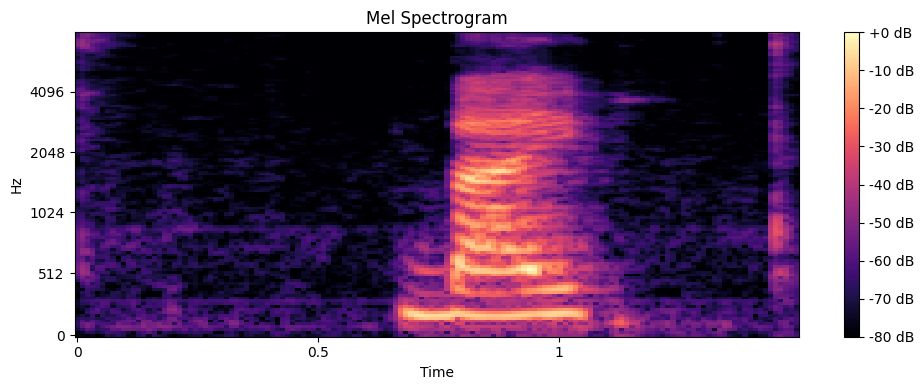
\includegraphics[width=0.5\textwidth]{Figures/Fig_NoiseBefore.png}}
    \caption{Spectrogram before noise reduction}
    \label{fig_NoiseBefore} % ``Fig.~\ref{fig_Noise}''
    \end{figure}

\begin{figure}[hbtp]
    \centerline{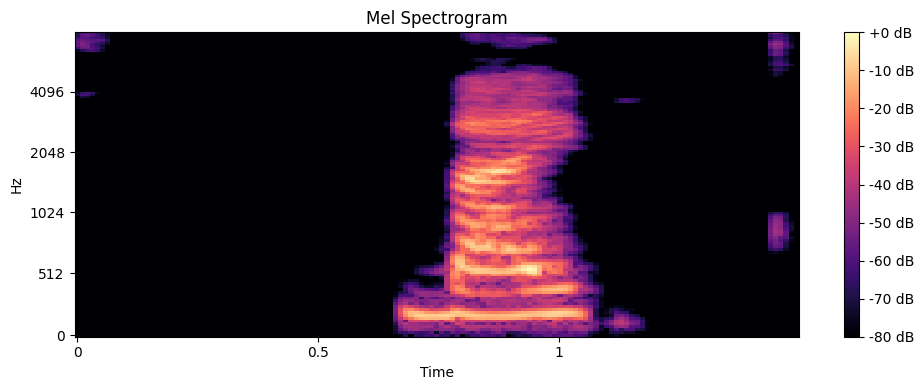
\includegraphics[width=0.5\textwidth]{Figures/Fig_NoiseAfter.png}}
    \caption{Spectrogram after noise reduction}
    \label{fig_NoiseAfter} % ``Fig.~\ref{fig_Noise}''
    \end{figure}

We normalized the volume to achieve voice intensity consistency. After the normalization the amplitude of audio signal does not exceed the range from \numrange[range-phrase =\text{ to }]{-1}{1}. For normalization we used the \textit{librosa.util.normalize} function.
We standardized the length of recordings by cutting and filling and balanced the representation of each class by equalizing the number of positive and negative samples.
We split the dataset into training, validation and test sets (in proportion of 0.7, 0.15, 0.15). We conducted data augmentation on the training set, which included altering speed and voice level of recordings using functions from \textit{librosa.effects} library.
After obtaining the spectrograms required as an input for our models, we observed a significant improvement in the training.

\subsection{CNN for Tone Recognition}
We used a multilayer CNN based on \cite{Gao2019ToneNetAC}. It classifies the tone of speech phonemes into one of 4 defined tones (1 to 4, not counting the neutral one, denoted by 0). The network consists of convolution layers, batch normalization, activation functions and pooling layers.
The input layer takes two-dimensional data and passes the output to 4 convolution blocks with the number of filters ascending through values: 64, 128, 256, 512 and altering steps, which allow hierarchical feature extraction. Finally we apply Data Flattening combined with 2 Fully Connected Layers (FCLs) of 1024 units followed by a softmax layer to obtain probabilities.
For this model we used the Stochastic gradient descent optimization algorithm \cite{sung2020ssgdsymmetricalstochasticgradient} with a low learning rate and special weights applied for classes with inconsistent representation in training data.
We used techniques of early stopping and saving checkpoints to avoid overfitting and ensure the best results are not lost.

\subsection{CNN for Pronunciation Evaluation}
For this task we used the numeric words from 0 to 10 and 100 from our Mandarin chinese audio dataset with labels provided by a native Chinese speaking expert in the field. For each word we trained a separate model, as the results for a single model trained on all the words haven't been satisfactory. The network takes a 3-channel spectrogram as an input. Similarly to our Tone Recognition model, the architecture is based on convolution and pooling layers.
The number of convolution filters grows to 128. Thanks to the MaxPooling layers, the model's number of trainable parameters is reduced, alleviating the computational cost and risk of overfitting. After extracting the features with convolutional blocks, we use a Flatten layer.
Afterwards the tensors are passed to FCLs with 1024 and 128 units in this order and ReLU activation function. In order to prevent overfitting we use a Dropout layer that randomly disables half of the neurons, improving the model's generalization capability.
In the end there is a 1-unit FCL with a sigmoid activation function, responsible for outputting a probability of given word, allowing binary classification. During the training we use the Adam optimizer \cite{Kingma2014AdamAM} with Binary Cross-Entropy loss function.
The hyperparameters we used for this model are summarized in ``Tab.~\ref{tab_CNNPE_hyper}''.

\begin{table}[hbtp]
    \caption{Pronunciation Evaluation - CNN hyperparameters}
    \begin{center}
    \begin{tabular}{|c|c|}
    \hline
    \textbf{Parameter} & {\textbf{Value}} \\
    \hline
    batch size & 32 \\
    \hline
    learning rate & 0.0001 \\
    \hline
    dropout & 0.2 \\
    \hline
    smoothing & 0.1 \\
    \hline
    \end{tabular}
    \label{tab_CNNPE_hyper}
    \end{center}
    \end{table}

\subsection{Speech-Transformer for complete ASR}
With this last model, using an implementation of \cite{vaswani2023attentionneed,8462506}, modified to enable training with \cite{shi2021aishell3multispeakermandarintts} and finetuning with our dataset, we attempted solving both tasks of Pronunciation Evaluation and Tone Classification.
Transformers have recently gained high popularity in Sequence-to-Sequence tasks such as Natural Language Processing. The architecture we used is based on Multi-Head Attention, which enables applying the attention mechanism in parallel, with separate learnable parameters. The Batch Normalization technique typical for CNNs, here has been replaced by Layer Normalization applied in each Encoder and Decoder layer.
The architecture is presented in more detail in ``Fig.~\ref{fig_STArch}''.

\begin{figure}[hbtp]
    \centerline{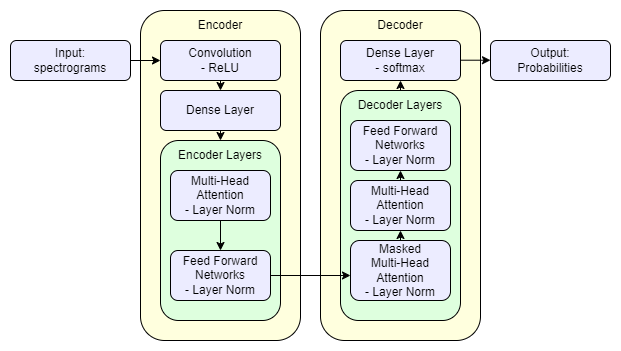
\includegraphics[width=0.5\textwidth]{Figures/Speech-Transformer.png}}
    \caption{Speech-Transformer Architecture}
    \label{fig_STArch} % ``Fig.~\ref{fig_Noise}''
    \end{figure}

The model would originally generate transcription sequences based on processed audio input. In case of Mandarin chinese, the transcription can be represented in traditional alphabet or in pinyin notation, which consists of syllables written with latin letters and denotes the tone of each phone.
The pinyin is popular for learning purposes for foreigners who don't know the Chinese alphabet. It also enables us to simply split the phoneme into pronunciation and tone information.
The model has been configured with default hyperparameter values as in \cite{8462506}. Due to lack of specific transcriptions in our dataset (we were limited to pronunciation scores and tone labels) the training split for the finetuning part had to be limited to correct recordings. % the minority unfortunately
For the testing, however, we used balanced amount of correct and incorrect recordings for pronunciation evaluation and all the recording for tone classification.

\section{Results}

\subsection{CNN for Tone Classification}

The accuracy initially achieved with our model was around 0.50. After data preprocessing we were able to raise that score to 0.57.
The results of this CNN are also presented in a form of a confusion matrix in 

\begin{figure}[hbtp]
    \centerline{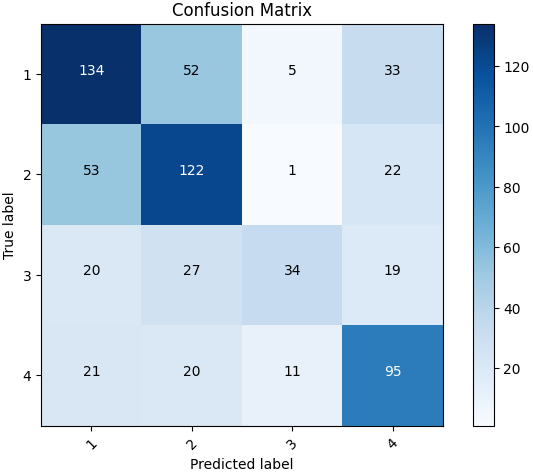
\includegraphics[width=0.5\textwidth]{Figures/ToneCNN_Matrix.png}}
    \caption{CNN }
    \label{fig_ToneCNN_Mat} % ``Fig.~\ref{fig_ToneCNN_Mat}''
    \end{figure}

\subsection{CNN - Confusion Matrix for Tone Classification}

The results of a model trained for each word are presented in ``Tab.~\ref{tab_CNNPE_acc}''.

\begin{table}[hbtp]
    \caption{CNN - Pronunciation Evaluation Metrics}
    \begin{center}
    \begin{tabular}{|c|c|}
    \hline
    \textbf{Word} & {\textbf{Accuracy}} \\
    \hline
    a0 & 0.78 \\
    \hline
    a1 & 0.77 \\
    \hline
    a2 & 0.67 \\
    \hline
    a3 & 0.61 \\
    \hline
    a4 & 0.73 \\
    \hline
    a5 & 0.72 \\
    \hline
    a6 & 0.69 \\
    \hline
    a7 & 0.68 \\
    \hline
    a8 & 0.70 \\
    \hline
    a9 & 0.70 \\
    \hline
    a10 & 0.71 \\
    \hline
    a100 & 0.73 \\
    \hline
    \textbf{Average} & \textbf{0.7075} \\
    \hline
    \end{tabular}
    \label{tab_CNNPE_acc}
    \end{center}
    \end{table}

% \subsection{Speech-Transformer - Pronunciation Evaluation}
\subsection{Speech-Transformer}
We measured this model with an accuracy metric. The results are given in the table ``Tab.~\ref{tab_STPE}''. We have also plotted a confusion matrix ``Fig.~\ref{fig_STPE}''.

\begin{table}[hbtp]
\caption{Speech-Transformer - Pronunciation Evaluation Metrics}
\begin{center}
\begin{tabular}{|c|c|}
\hline
\textbf{Metric} & {\textbf{Value}} \\
% \cline{2-4} 
% \textbf{Head} & \textbf{\textit{Table column subhead}}& \textbf{\textit{Subhead}}& \textbf{\textit{Subhead}} \\
\hline
Tone Classification Accuracy & 0.48 \\
\hline
Articulation Scoring Accuracy & 0.85 \\
\hline
\end{tabular}
\label{tab_STPE}
\end{center}
\end{table}

\begin{figure}[hbtp]
\centerline{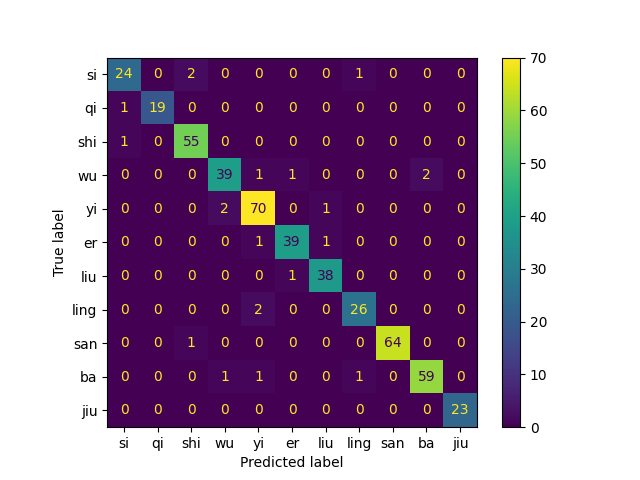
\includegraphics[width=0.5\textwidth]{Figures/Fig_STPE.png}}
\caption{Speech-Transformer - Confusion Matrix for PE}
\label{fig_STPE} % ``Fig.~\ref{fig_STPE}''
\end{figure}

% \subsection{Speech-Transformer - Tone Classification}
Before the finetuning, this model would achieve at most 50\% accuracy, meaning half of the times it would guess one of the 4 available tones (excluding the neutral tone).
Afterwards it actually dropped below that value, because it was not trained separately for this task and two tones out of four are underrepresented within the numeric words from 1 to 10, which can be observed on a confusion matrix ``Fig.~\ref{fig_STTC}''.

\begin{figure}[hbtp]
    \centerline{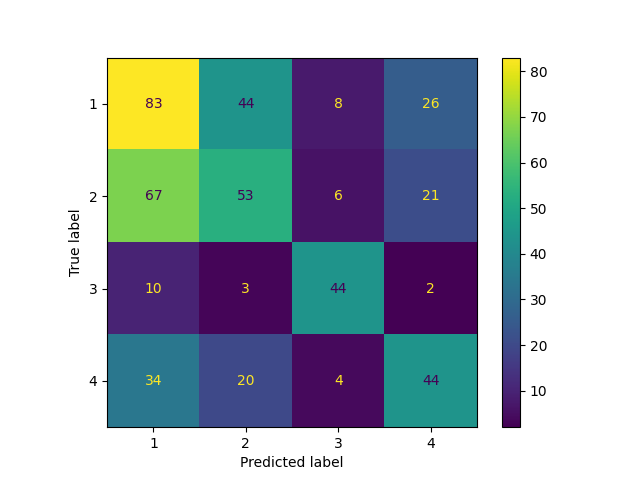
\includegraphics[width=0.5\textwidth]{Figures/Fig_STTC.png}}
    \caption{Speech-Transformer - Confusion Matrix for TC}
    \label{fig_STTC}
\end{figure}

\section{Discussion}
In the Pronunciation Scoring task, the Speech-Transformer has achieved a noticeably higher accuracy. Apart from significant difference of these networks, the Speech-Transformer has been pre-trained with \cite{shi2021aishell3multispeakermandarintts}. At this stage of research, accuracy of over 0.70 for a ten class problem is not a bad score. Ideally, the same result would be achieved with a single CNN for all the words.
Another improvement would be to support multi-syllable words, which is currently possible only with the use of the Speech-Transformer as it's a sequence-processing-oriented approach.
As per Tone Classification, the CNN has outperformed the Speech-Transformer. It's worth to note that in both cases the first two tones were likely to get confused. This can be observed in the upper-left corner of both ``Fig.~\ref{fig_ToneCNN_Mat}'' and ``Fig.~\ref{fig_STTC}''. Unfortunately, even the accuracy of the CNN, which scored 0.57, can't be considered a success given there are only 4 tones to classify. To achieve a higher accuracy with our proposed models, it might be necessary to acquire more training data, enhance the data processing techniques, balance the tone samples in the dataset and remove the ones with any uncertainty (based on the confusion of both our models around the first two tones).

\section{Conclusion}
The Pronunciation Scoring accuracy of our models shows that it's in fact possible to achieve results comparable to human experts in the field. Although the Tone Classification task hasn't been accomplished at the same level, it's certainly within the reach of our successors given some enhancements listed in the previous paragraph are there to be made.

% \subsection{Some Common Mistakes}\label{SCM}
% \begin{itemize}
% \item The word ``data'' is plural, not singular.
% \item The subscript for the permeability of vacuum $\mu_{0}$, and other common scientific constants, is zero with subscript formatting, not a lowercase letter ``o''.
% \item In American English, commas, semicolons, periods, question and exclamation marks are located within quotation marks only when a complete thought or name is cited, such as a title or full quotation. When quotation marks are used, instead of a bold or italic typeface, to highlight a word or phrase, punctuation should appear outside of the quotation marks. A parenthetical phrase or statement at the end of a sentence is punctuated outside of the closing parenthesis (like this). (A parenthetical sentence is punctuated within the parentheses.)
% \item A graph within a graph is an ``inset'', not an ``insert''. The word alternatively is preferred to the word ``alternately'' (unless you really mean something that alternates).
% \item Do not use the word ``essentially'' to mean ``approximately'' or ``effectively''.
% \item In your paper title, if the words ``that uses'' can accurately replace the word ``using'', capitalize the ``u''; if not, keep using lower-cased.
% \item Be aware of the different meanings of the homophones ``affect'' and ``effect'', ``complement'' and ``compliment'', ``discreet'' and ``discrete'', ``principal'' and ``principle''.
% \item Do not confuse ``imply'' and ``infer''.
% \item The prefix ``non'' is not a word; it should be joined to the word it modifies, usually without a hyphen.
% \item There is no period after the ``et'' in the Latin abbreviation ``et al.''.
% \item The abbreviation ``i.e.'' means ``that is'', and the abbreviation ``e.g.'' means ``for example''.
% \end{itemize}
% An excellent style manual for science writers is \cite{b7}.

% \subsection{Figures and Tables}
% \paragraph{Positioning Figures and Tables} Place figures and tables at the top and 
% bottom of columns. Avoid placing them in the middle of columns. Large 
% figures and tables may span across both columns. Figure captions should be 
% below the figures; table heads should appear above the tables. Insert 
% figures and tables after they are cited in the text. Use the abbreviation 
% ``Fig.~\ref{fig}'', even at the beginning of a sentence.

% \begin{table}[htbp]
% \caption{Table Type Styles}
% \begin{center}
% \begin{tabular}{|c|c|c|c|}
% \hline
% \textbf{Table}&\multicolumn{3}{|c|}{\textbf{Table Column Head}} \\
% \cline{2-4} 
% \textbf{Head} & \textbf{\textit{Table column subhead}}& \textbf{\textit{Subhead}}& \textbf{\textit{Subhead}} \\
% \hline
% copy& More table copy$^{\mathrm{a}}$& &  \\
% \hline
% \multicolumn{4}{l}{$^{\mathrm{a}}$Sample of a Table footnote.}
% \end{tabular}
% \label{tab1}
% \end{center}
% \end{table}

% \begin{figure}[hbtp]
% \centerline{\includegraphics{fig1.png}}
% \caption{Example of a figure caption.}
% \label{fig}
% \end{figure}

% Figure Labels: Use 8 point Times New Roman for Figure labels. Use words 
% rather than symbols or abbreviations when writing Figure axis labels to 
% avoid confusing the reader. As an example, write the quantity 
% ``Magnetization'', or ``Magnetization, M'', not just ``M''. If including 
% units in the label, present them within parentheses. Do not label axes only 
% with units. In the example, write ``Magnetization (A/m)'' or ``Magnetization 
% \{A[m(1)]\}'', not just ``A/m''. Do not label axes with a ratio of 
% quantities and units. For example, write ``Temperature (K)'', not 
% ``Temperature/K''.

\bibliographystyle{IEEEtran}
\bibliography{IEEE_references.bib}

\end{document}
